\documentclass[conference]{IEEEtran}

\ifCLASSINFOpdf
  % \usepackage[pdftex]{graphicx}
  % declare the path(s) where your graphic files are
  % \graphicspath{{../pdf/}{../jpeg/}}
  % and their extensions so you won't have to specify these with
  % every instance of \includegraphics
  % \DeclareGraphicsExtensions{.pdf,.jpeg,.png}
\else
  % or other class option (dvipsone, dvipdf, if not using dvips). graphicx
  % will default to the driver specified in the system graphics.cfg if no
  % driver is specified.
  % \usepackage[dvips]{graphicx}
  % declare the path(s) where your graphic files are
  % \graphicspath{{../eps/}}
  % and their extensions so you won't have to specify these with
  % every instance of \includegraphics
  % \DeclareGraphicsExtensions{.eps}
\fi

\usepackage[utf8]{inputenc}
\usepackage{graphicx}
\usepackage[T1]{fontenc}
\usepackage[hyphens]{url}
\usepackage{listings}
\usepackage{textcomp}
\lstset{
        basicstyle=\ttfamily\scriptsize,
        upquote=true,
        showspaces=false,
        showstringspaces=false,
        showtabs=false,
        tabsize=2,
        frame=none,
        breaklines,
        numbers=none,
        framexleftmargin=2mm,
        xleftmargin=2mm,
}

%% Define a new 'smallurl' style for the package that will use a smaller font.
\makeatletter
\def\url@smallurlstyle{%
  \@ifundefined{selectfont}{\def\UrlFont{\sf}}{\def\UrlFont{\scriptsize\ttfamily}}}
\makeatother
%% Now actually use the newly defined style.
\urlstyle{smallurl}
\newcommand{\nofootnote}[1]{~#1}

% correct bad hyphenation here
\hyphenation{op-tical net-works semi-conduc-tor}

\begin{document}
%
% paper title
% can use linebreaks \\ within to get better formatting as desired
\title{Adding Meaning to Facebook Microposts Via A Mash-up API And Tracking Its Data's Provenance}

% author names and affiliations
% use a multiple column layout for up to three different
% affiliations
\author{\IEEEauthorblockN{Thomas Steiner}
\IEEEauthorblockA{Univ. Politècnica de Catalunya\\
Department LSI\\
08034 Barcelona, Spain\\
Email: tsteiner@lsi.upc.edu}
\and
\IEEEauthorblockN{Ruben Verborgh}
\IEEEauthorblockA{Ghent University – IBBT\\
ELIS – Multimedia Lab \\
B-9050 Ledeberg-Ghent, Belgium\\
Email: ruben.verborgh@ugent.be}
\and
\IEEEauthorblockN{Joaquim Gabarr\'{o} Vall\'{e}s}
\IEEEauthorblockA{Univ. Politècnica de Catalunya\\
Department LSI\\
08034 Barcelona, Spain\\
Email: gabarro@lsi.upc.edu}}

% make the title area
\maketitle

\begin{abstract}
%\boldmath
The social networking website Facebook offers to its users a feature called ``status updates" (or just ``status"), which allows for users to create microposts directed to all, or a subset of their contacts. Readers can respond to microposts, or in addition to that also click a ``Like" button to show their appreciation for a certain micropost. Adding semantic meaning in the sense of unambiguous intended ideas to such microposts can, for example, be achieved via Natural Language Processing (NLP). Therefore, we have implemented a RESTful mash-up NLP API based on a combination of several third party NLP APIs in order to retrieve more accurate results in the sense of emergence. In consequence, our API uses third party APIs opaquely in the background in order to deliver its output. In this paper, we describe how one can keep track of provenance and credit back the contributions of each single API to the combined result of all APIs. The main contribution of our work is a description of how provenance metadata can be automatically added to the output of mash-up APIs like the one presented in this paper.
\end{abstract}

\IEEEpeerreviewmaketitle

\section{Introduction}                                                      \label{sec:introduction}
According to official Facebook statistics~\cite{Facebook}, the social networking website has more than 500 million active users out of which half log on to Facebook in any given day. The average Facebook user has 130 friends, and creates 90 pieces of content each month. This sums up to the impressive number of overall twenty-two billion five hundred million pieces of content per month. Similar to the microblogging website Twitter with its full text Twitter search\footnote{\url{https://search.twitter.com/}}, Facebook as well offers both a search feature on the website, and a JSON-based search API over status updates from all global Facebook members\footnote{Sample Facebook search for ``salamanca, spain": \url{https://graph.facebook.com/search?q=salamanca,\%20spain&type=post}}. In order to perform data mining, a statistically significant amount of microposts is necessary (this is also known as access to the ``firehose"). However, while Twitter grants selected parties access to its Streaming API~\cite{Twitter} for that purpose, for Facebook there is no such documented option. To address this shortage, we have developed a Google Chrome browser extension called Facebook Swarm NLP.

The Facebook Swarm NLP extension\footnote{\url{https://chrome.google.com/webstore/detail/nhcgonkeclhijbkpelhmclmjijphafhk}} first injects JavaScript code into the Facebook.com homepage to perform data analysis on the encountered set of microposts, and then sends the results to a central data processing point. Given a broad enough installation base, this extension allows for a random sample of microposts to be analyzed as they become available on Facebook -- in effect a very modest firehose. The extension first checks if the user is logged in to Facebook.com, and if so, retrieves all status updates from the contacts that are displayed on the current user's Facebook homepage. Second, the extension performs named entity extraction via Natural Language Processing (NLP) using a remote NLP API on each of these status updates in order to add semantic meaning to them. The extracted named entities are then displayed below each post, as illustrated in Figure~\ref{fig:facebook}. Finally the extracted named entities are sent to a central Google Analytics~\cite{Kaushik} profile to compute basic or advanced trends, for example by ranking the most discussed-about named entities per day, or by pivoting named entities by Analytics data, like users' geographic locations.

\begin{figure}[htb!]
  \centering
    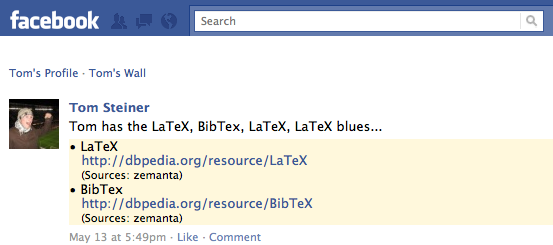
\includegraphics[width=0.45\textwidth]{facebook-swarm-nlp.png}
  \caption{Facebook Swarm NLP Chrome extension. Extracted named entities have a pale yellow background.}     
  \label{fig:facebook}
\end{figure}

As mentioned before, in order to perform named entity extraction, we rely on a mash-up API that calls existing third party NLP APIs in the background, and that delivers the combined results of these APIs in a consolidated way. Obviously it is very desirable (i) to credit back the contribution of each single third party API to the joint results, and (ii) to track the provenance of the joint results in order to understand how they were formed. We will show at the concrete example of the mash-up NLP API used for our Facebook Swarm NLP extension how these two constraints can be fulfilled in a generalizable way.

The remainder of this paper is structured as follows: We discuss related work in Section~\ref{sec:related}. In Section~\ref{sec:services}, we introduce APIs that allow for unstructured data to be converted into Linked Data. In Section~\ref{sec:tracking}, we describe how we automatically maintain provenance metadata in our API. Section~\ref{sec:future} presents Future Work. Finally Section~\ref{sec:conclusion} ends the paper with a Conclusion.

\section{Related Work}\label{sec:related}
In~\cite{Groth:2009:MPD:1462159.1462162}, Groth et al. describe how through tools and technologies such as Yahoo Pipes, Really Simple Syndication (RSS) and APIs, so-called mash-ups can be created in a dynamic, just-in-time way, combining data from different data sources. The authors are driven by the motivation to allow for trust and confidence in mash-ups, and therefore consider it critical to be able to analyze the origin of combined results. They suggest an approach based on OWL and XML, with a focus on process documentation. However, different from us, where the goal is to transparently add provenance data at API invocation level, there focus is more on overall process documentation in the context of a mash-up application.

The focus of Carroll et al. in~\cite{carroll2005} is on the provenance of triples in the Semantic Web world, namely, for making statements about triples in graphs, therefore the paper introduces the concept of named graphs, an extension to RDF. In contrast to our work, Carroll et al. focus purely on using triples to make statements about triples (that is, they stay in the RDF world), whereas our approach uses RDF to make statements about potentially any API result, that is, our approach is not limited to RDF results, albeit in the concrete case we use RDF in addition to JSON as such API result.

In the WS-* world, BPEL4WS, described by Curbera et al. in~\cite{Curbera:2003:NSW:944217.944234} provides a formal language for the specification of business processes and business interaction protocols. This allows for the combination of several APIs, however, does not credit back concrete outputs of a combined API to the underlying APIs.

\section{APIs for converting unstructured data into Linked Data}    \label{sec:services}
Sir Tim Berners-Lee has introduced Linked Data~\cite{TimBL:LinkedData} in a W3C Design Issue, where he defines the four rules for Linked Data:
\begin{enumerate}
\item Use URIs as names for things.
\item Use HTTP URIs so that people can look up those names.
\item When someone looks up a URI, provide useful information, using the standards (RDF*, SPARQL).
\item Include links to other URIs, so that they can discover more things.
\end{enumerate}
In order to represent extracted named entities from Facebook microposts in an unambiguous way, we apply the first and the second Linked Data principle by representing named entities with HTTP URIs. This is taken care of by the third party NLP APIs that we use for our Chrome extension, namely OpenCalais~\cite{OpenCalais}, Zemanta~\cite{Zemanta}, DBpedia Spotlight~\cite{Spotlight}, and AlchemyAPI~\cite{AlchemyApi}. These APIs take a text fragment as an input, perform named entity extraction on it, and then link the extracted entities back into the Linking Open Data (LOD) cloud\footnote{\url{http://lod-cloud.net/}}. We use these APIs in parallel, and by combining their results aiming at the emergence effect in the sense of Aristotle: ``\emph{[\ldots] the totality is not, as it were, a mere heap, but the whole is something besides the parts [\ldots]}''\footnote{Aristotle, Metaphysics, Book H 1045a 8-10.}. 

\subsection{Combining Results from Different NLP APIs}                     \label{sec:consolidation-nlp}
We have implemented a mash-up API for the four NLP APIs. While the original calls to each particular NLP API are all HTTP \texttt{POST}-based, we have implemented the mash-up API \texttt{GET}- and \texttt{POST}-based. All NLP APIs return entities with their types and/or subtypes, names, relevance, and URIs that link into the LOD cloud. Our mash-up API supports two output formats, namely /application/json and /text/turtle (an RDF~\cite{RDF} serialization format). The combined output in JSON form for the micropost ``Tom has the LaTeX, BibTeX, LaTeX, LaTeX blues...'' (see Figure~\ref{fig:facebook}) is shown below:
\begin{lstlisting}
[
  {
    "name": "LaTeX",
    "relevance": 0.7128319999999999,
    "uris": [
      {
        "uri": "http://dbpedia.org/resource/LaTeX",
        "source": "zemanta"
      }
    ],
    "source": "zemanta"
  },
  {
    "name": "BibTeX",
    "relevance": 0.8143277777777777,
    "uris": [
      {
        "uri": "http://dbpedia.org/resource/BibTeX",
        "source": "zemanta"
      }
    ],
    "source": "zemanta"
  }  
]
\end{lstlisting}

These joint results come from a request to our mash-up API via \texttt{GET} \url{/entity-extraction/combined/Tom%20has%20the%20LaTeX%2C%20BibTeX%2C%20LaTeX%2C%20LaTeX%20blues...}.

\subsection{The Need for Providing Provenance Metadata}
Hartig et al. mention in~\cite{ipaw10:olaf} some reasons that justify the need for provenance metadata. Among those, linked dataset replication and distribution on the Web with not necessarily always the same namespaces: based on the same source data, different copies of a linked dataset can be created with different degrees of interconnectedness by different publishers.

We add to this list the automatic conversion of legacy unstructured data to Linked Data with heuristics where extracted entities -- while being consolidated and backed up by different data sources -- might still be wrong. Especially with our ``mash-up''-like approach, it is very desirable to be able to track back to the concrete source where a certain piece of information might have come from. This enables (i) to correct the error at the root of our API (fighting the cause), (ii) to correct the concrete error in an RDF annotation (fighting the symptom), and (iii) to judge the trustworthiness and quality of a dataset which is probably the most important reason.

\section{Tracking Provenance With Multiple Data Sources}                    \label{sec:tracking}
As outlined before, we use several data sources (APIs) in the background in order to add meaning to Facebook microposts. Extracted named entities from a Facebook micropost might in consequence be the result of up to four agreeing (or disagreeing) API calls (see Section~\ref{sec:services}). In order to track the contributions of the various sources, we have decided to use the Provenance Vocabulary~\cite{Hartig:Provenance} by Hartig and Zhao with the prefix \texttt{prv}, the HTTP Vocabulary in RDF~\cite{HTTP:RDF} by Koch et al. with prefix \texttt{http}, and a vocabulary for Representing Content in RDF~\cite{CNT:RDF} by the same authors with prefix \texttt{cnt}. We have chosen the HTTP Vocabulary in RDF for the fact that it is a W3C Working Draft  developed by the Evaluation and Repair Tools Working Group (ERT WG), which is part of the World Wide Web Consortium (W3C) Web Accessibility Initiative (WAI). The Provenance Vocabulary was chosen because of its relatively broad implementation in several projects, such as Pubby\footnote{\url{http://www4.wiwiss.fu-berlin.de/pubby/}}, Triplify\footnote{\url{http://triplify.org/Overview}}, and D2R Server\footnote{\url{http://www4.wiwiss.fu-berlin.de/bizer/d2r-server/}}.

While our mash-up API supports two output formats (/application/json and /text/turtle), we have added provenance information exclusively to the /text/turtle variant. In order to represent the extracted named entities in a Facebook micropost, we use the Common Tag vocabulary~\cite{CommonTag:Spec}. A micropost is \url{ctag:tagged} with a \url{ctag:Tag}, which consists of a textual \url{ctag:label} and a pointer to a resource that specifies what the label \url{ctag:means}. The Common Tag vocabulary is well-established and developed by both industry and academic partners. In order to make statements about a bundle of triples, we group them in a named graph. We use the TriG~\cite{Bizer:TriG} syntax:
\begin{lstlisting}
:G = {
  <https://www.facebook.com/Tomayac/posts/10150177486072286> ctag:tagged [
      a ctag:Tag ;
      ctag:label "BibTeX" ;
      ctag:means <http://dbpedia.org/resource/BibTeX>
    ] .
} .
\end{lstlisting}

\subsection{The Provenance Vocabulary}                                      \label{sec:provenance}
In this section, we outline the required steps in order to make statements about the provenance of a group of triples contained in a named graph \url{:G} that was generated using several HTTP \texttt{GET} requests to third party APIs. We use the Provenance Vocabulary~\cite{Hartig:Provenance} with the prefix \texttt{prv}, the HTTP Vocabulary in RDF~\cite{HTTP:RDF} with prefix \texttt{http}, and the Representing Content in RDF~\cite{CNT:RDF} vocabulary with prefix \texttt{cnt}.

First, we state that \url{:G} is both a \url{prv:DataItem} and obviously an \url{rdfg:Graph}. \url{:G} is \url{prv:createdBy} the process of a \url{prv:DataCreation}. This \url{prv:DataCreation} is \url{prv:performedBy} a \url{prv:NonHumanActor}, a \url{prvTypes:DataCreatingService} to be precise. This service is \url{prv:operatedBy} a human (\url{http://tomayac.com/thomas_steiner.rdf#me}). Time is often important for provenance, so the \url{prv:performedAt} date of the \url{prv:DataCreation} needs to be saved. During the process of the \url{prv:DataCreation} there are \url{prv:usedData}, which are \url{prv:retrievedBy} a \url{prv:DataAcess} that is \url{prv:performedAt} a certain time, and \url{prv:performedBy} a non-human actor (our API) that is \url{prv:operatedBy} a human (\url{http://tomayac.com/thomas_steiner.rdf#me}. For the \url{prv:DataAccess} (there is one for each third party API involved), we \url{prv:accessedService} from a \url{prv:DataProvidingService} of which we \url{prv:accessedResource} at a certain \url{irw:WebResource}. Therefore, we \url{prvTypes:exchangedHTTPMessage} which is an \url{http:Request} using \url{http:httpVersion} ``1.1'' and the \url{http:methodName} ``GET''.

\subsection{Provenance RDF Overview}                                           \label{sec:appendix}
This section provides a shortened overview of the provenance RDF in Turtle syntax for a Facebook micropost tagged with the label ``BibTeX'' and the assigned
meaning \url{http://dbpedia.org/resource/BibTeX}. The named graph \url{:G} in the first part of the listing contains the absolute data (the fact that the Facebook micropost with the URI \url{https://www.facebook.com/Tomayac/posts/10150177486072286} is tagged with the label ``BibTeX", which is represented by the HTTP URI \url{http://dbpedia.org/resource/BibTeX}). The second part with metadata about \url{:G} says that these facts were generated via two calls, one using the HTTP method \texttt{GET}, and the other \texttt{POST}:
\begin{lstlisting}
:G = {
  <https://www.facebook.com/Tomayac/posts/10150177486072286> ctag:tagged [
     a ctag:Tag ;
     ctag:label "BibTeX" ;
     ctag:means <http://dbpedia.org/resource/BibTeX> ;
} .

:G
  a prv:DataItem ;
  a rdfg:Graph ;
  prv:createdBy [
    a prv:DataCreation ;
    prv:performedAt "2011-05-01T12:42:30Z"^^xsd:dateTime ;
    prv:performedBy [
      a prv:NonHumanActor ;
      a prvTypes:DataCreatingService ;
      prv:operatedBy <http://tomayac.com/thomas_steiner.rdf#me> .
    ] ;
    prv:usedData [
      prv:retrievedBy [
        a prv:DataAcess ;
        prv:performedAt "2011-05-18T12:42:30Z"^^xsd:dateTime ;
        prv:performedBy [
          prv:operatedBy <http://tomayac.com/thomas_steiner.rdf#me> .
        ] ;
        prv:accessedService <http://spotlight.dbpedia.org/rest/annotate> ;
        prv:accessedResource <http://spotlight.dbpedia.org/rest/annotate?text=Tom%20has%20the%20LaTeX%2C%20BibTeX%2C%20LaTeX%2C%20LaTeX%20blues...&confidence=0.4&support=20> ;
        prvTypes:exchangedHTTPMessage [
          a http:Request ;
          http:httpVersion "1.1" ;
          http:methodName "GET" ;
          http:mthd <http://www.w3.org/2008/http-methods#GET> ;
          http:headers (
            [
              http:fieldName "Host" ;
              http:fieldValue "spotlight.dbpedia.org" ;
              http:hdrName <http://www.w3.org/2008/http-header#host> ;
            ]
          )
        ] ;
      ] ;
    ] ;
    prv:usedData [
      prv:retrievedBy [
        a prv:DataAcess ;
        prv:performedAt "2011-05-18T12:42:30Z"^^xsd:dateTime ;
        prv:performedBy [
          prv:operatedBy <http://tomayac.com/thomas_steiner.rdf#me> .
        ] ;
        prv:accessedService <http://api.zemanta.com/services/rest/0.0/> ;
        prv:accessedResource <http://api.zemanta.com/services/rest/0.0/> ;
        prvTypes:exchangedHTTPMessage [
          a http:Request ;
          http:httpVersion "1.1" ;
          http:methodName "POST" ;
          http:mthd <http://www.w3.org/2008/http-methods#POST> ;
          http:headers (
            [
              http:fieldName "Host" ;
              http:fieldValue "api.zemanta.com" ;
              http:hdrName <http://www.w3.org/2008/http-header#host> ;
            ],
            [
              http:fieldName "Content-Type" ;
              http:fieldValue "application/x-www-form-urlencoded" ;
            ],
            [
              http:fieldName "Connection" ;
              http:fieldValue "close" ;
            ]   
          )
          http:body [
            cnt:ContentAsText [
              cnt:characterEncoding "UTF-8" ;
              cnt:chars """method=zemanta.suggest_markup
              &api_key=4eqem8kyjzvkz8d2ken3xprb
              &text=Tom%20has%20the%20LaTeX%2C%20BibTeX%2C%20LaTeX%2C%20LaTeX%20blues...
              &format=json
              &return_rdf_links=1""" ;
            ] ;
          ] ;
        ] ;
      ] ;
    ] ;
  ] .
} .
\end{lstlisting}

It is to be noted that statements such as in the listing above refer to the triple objects as an identifier for a Web resource (where the Web resource is a representation of the result of the API call at the time where it was \url{prv:performedAt}). As provenance metadata always refer to the time context in which a certain statement was made, it is essentially unimportant what representation the resource returns at a later time.

\section{Future Work} \label{sec:future}
Already commenced future work will be to explore ways to stick to existing standards such as the HTTP in RDF and the Provenance vocabularies on the one hand, but on the other hand to simplify drastically in order to come to less verbose provenance descriptions. While it is always easier to come up with a specialized vocabulary that does one task well (for example we could imagine a simple vocabulary with the sole purpose to log the API call of an API invocation), broader reuse and acceptance can be gained by reusing existing vocabularies. We will investigate how to find the right balance here.

\section{Conclusion}                                                        \label{sec:conclusion}
We have introduced an API for adding semantic meaning to Facebook microposts. As mash-up data sources for our API we have presented NLP APIs, and then focused on the necessary RDF vocabularies to annotate Facebook microposts with the thereof extracted named entities in the form of common tags. Due to their different ``mash-up''-like history of origins, we need to track provenance metadata in order to assure the trustworthiness of the generated data. We showed how the Provenance Vocabulary can be used to keep track of the original third party API calls that led to the consolidated results. We have shown how a concrete multi-source RESTful API can automatically maintain provenance metadata. We believe that being able to track back the origin of a piece of data is of crucial importance, however, the generated provenance-related triples are very verbose, and in consequence stating even simple facts like that a combined result is based on two separate sub-results takes up a lot of space. The verbosity is mainly due to the used vocabularies, the Provenance Vocabulary and the HTTP Vocabulary in RDF. We are conscious that our current approach is a first step in the right direction, however, that some more steps are ahead to take. Our vision is to establish a common method for specifying provenance data for mash-up APIs.

% conference papers do not normally have an appendix

% use section* for acknowledgement
\section*{Acknowledgment}

This work was partly supported by the European Commission under Grant No. 248296 FP7 I-SEARCH project.

\bibliographystyle{abbrv}
\bibliography{nwesp2011}

\end{document}